\chapter{Physical model}
\label{chap:Chapter-2}
\textit{In this chapter, it's exposing the fundamental physics to understand the experimental results' trough physical model, both numerical and phenomenological. It is emphasis in symmetry properties of semiconductors, which is the base to get our model.}
\vfill
\minitoc
\newpage

\lettrine[lines=3, lraise=.1, nindent=0mm, slope=0mm]{\textbf{S}}{emiconductors} are alloy of materials with pare structural characteristics, it's the alloys which can generates an amazing quantum process that is quantum confinement.  But, all of them  couldn't possibly be achieved with understand of semiconductor bands, are bands the reason to get semiconductor heterostructures. Now, the objective is proposing the model to study Coupled Quantum Wells. The CQWs are heterostructures grown from a semiconductor substrate as GaAs as previous treated SQW (see \Cref{fig:subsection-1.2-single-quantum-well-scheme}) but coupled by a thin barrier which have a very significant role. But before to mention the objective of study this structures and the physical model which explain their experimental results  is important to call about of the symmetry and their relevance to understand the physics of these QS. \\*
Previously,  we were very repeating in the importance of semiconductor band structure, also to  in remark difficult of get them. It was saying the complexity of calculate semiconductor bands is high, by this reason it's developed models to approximate it. But, all of these couldn't be possible if it would not be taken into account the \emph{symmetry} role in physics\cite{van1989laws}. Thanks to symmetry, it's possible to understand from Quantum to Universe. It is clear that to talk the symmetry is inevitable to think in geometry or nature patterns  inherently way, but in the next sections it's established the symmetry role from the band structure calculation to  the importance in the electron behavior in CQWs structures. 




\section{The Symmetry Context}
\label{sec:chapter-2-from-symmetry}
\vspace{-10mm}
Talk about \emph{symmetry} is talk of shapes or in a romanticism way as  the natural harmony that makes something appear beautiful to us\cite{powell2010symmetry,tapp2021symmetry}. But, what is the reason the \emph{symmetry} is very important in physics?. The reason the  \emph{symmetry} is very important has to do with a \emph{transformation}, this mean that if a physical system is affected or perturbed by a thing and this appears to be exactly the same before and after that \emph{transformation}, it is said to be
\emph{invariant} under that \emph{transformation}. The symmetry of the system is made up of all the transformation operations that leave the system invariant\cite{powell2010symmetry}.

In this section doesn't have the purpose to be a one more copy or re-interpreted version of a group theory book, yes,  the group theory not symmetry theory, it's important to remember that to understand of symmetry physics of solids it's important to understand the group concept. 
In generally, a group is a set or collection of elements that obey certain criteria and are related to each other through a specific rule of interaction and obey four group axioms\cite{powell2010symmetry,cornwell1997group,muller2013symmetry}. 
It is important to remark which the heterostructure to will study is composed by GaAs/\algaas semiconductors, then  we started with the GaAs crystal to propound the symmetry role in the  CQWs.  Then, already raised the starting point,  remember that the crystal solid  can be defined as an  arrangement of atoms in strictly periodic arrays\cite{kittel2018kittel,solyom2007fundamentals}, from here arises two concepts: basis and lattice, where that last is the set of mathematical points to which the basis is attached\cite{kittel2018kittel}. These crystal concepts give place of crystal primitive cell in three dimensions also considered as the seed to reproduce a crystal. So, it gets  fundamental types of lattices defined  by a collection of \emph{symmetry} operations (rotation, translation etc.), then it's compose a lattice point group. In the three-dimensional case, the point symmetry groups require the 14 different lattices types\footnote{This lattices are known as Bravais Lattices}, where are classified into seven systems. Into these systems it's found the \emph{cubic} system, it which posses three number of lattices. Remember that the GaAs crystal is \emph{cubic},  specifically, is the type FCC lattice.  The FCC lattice is easy to imagine, if place an atom in each corner of  a cube and in a center of each face of it. Therefore, it is easier  to define  the planes and crystal directions if we take the cube faces as a reference it gets $(hkl)$ plane and the directions $\left[hkl\right]$ which must be perpendicular to a plane $(hkl)$\cite{kittel2018kittel}. 
\begin{figure}[h!]
	\centering
	\begin{subfigure}{\textwidth}
		\includegraphics[width=\linewidth]{../figures/chapter-2/symmetry/out/sym-0}
		\phantomsubcaption\label{subfig:subsubsection-2.1-crystal-rspace-a)}
		\phantomsubcaption\label{subfig:subsubsection-2.1-crystal-kspace-b)}
	\end{subfigure}
	\caption{\subref{subfig:subsubsection-2.1-crystal-rspace-a)} GaAs crystal structure in ``real space'',  this region is known as \emph{unit cell}, into that with dashed line is denoted the primitive cell. This lattice is well-defined by the vectors $\mathbf{a}$, $\mathbf{b}$ and $\mathbf{c}$, these vectors are defined as the basis vectors.  In \subref{subfig:subsubsection-2.1-crystal-kspace-b)} is schematized the GaAs crystal structure in $\boldsymbol{k}-$space, also known as \emph{reciprocal space}.}
	\label{fig:subsubsection-2.1-crystal-r-k-space}
\end{figure}

The lattice is an array of points which make the space lattice of a \cry and the repetitions or disposition of these points is controlled by ``\sym operations''\cite{chatterjee2008crystallography}. The crystal is composed by a space lattice this is a plane lattice\footnote{2D point pattern array} which have three \sym operations: \emph{Rotation axes}, \emph{Mirror plane} and \emph{Centre of Symmetry}. If add a one dimension to plane lattice it gets a space lattice, which define the unit cell of a \cry, so this adds one more \sym operation which is \emph{Rotation Inversion} or \emph{Roto-Inversion}. Then, can get \sym elements of a \cry if  apply the four \sym operations and their possible combinations. If collect that \sym elements obtains the \emph{point symmetry} or the \emph{point group of symmetry} of a \cry. 
The GaAs crystal as before mentioned is a \emph{cubic} system, but have a defined $cubic$ structure  called  as \emph{cubic zinc sulfide} or simply \emph{zincblende}. This specific \emph{cubic} structure  is characterized by arrangement of two type atoms with places  coordinates: $000$, $0\frac{1}{2}\frac{1}{2}$,  $\frac{1}{2} 0\frac{1}{2}$ , $\frac{1}{2} \frac{1}{2} 0$ for one type of these as Zn in ZnS or Ga in GaAs structure. In case of the second one atom, it has coordinates : $\frac{1}{4},\frac{1}{4},\frac{1}{4}$, $\frac{1}{4},\frac{3}{4},\frac{3}{4}$, $\frac{3}{4},\frac{1}{4}, \frac{3}{4}$, $\frac{3}{4},\frac{3}{4},\frac{1}{4}$ for S in ZnS or As in GaAs\cite{kittel2018kittel,mckelvey1966solid}.   The \Cref{subfig:subsubsection-2.1-crystal-rspace-a)} shows the unit cell of GaAs structure and into them it  dashed the primitive cell for the FCC lattice, also denoted the basis vectors  $\mathbf{a}$, $\mathbf{b}$ and $\mathbf{c}$.

In the case of symmetry of GaAs crystal, is important to remark that this symmetry can also denote in Hermann-Maguin notation  $F\overline{4}3m$ which corresponds to three fourfold rotary inversion parallel to the edges of a cube, with four threefold rotation axes parallel to the body diagonal and six mirror planes, each containing a face diagonal\cite{chatterjee2008crystallography}. The $F$ label corresponds to cubic system FCC, following by the corresponds operations.  \\*
The symmetry context before exposed can view as a macroscopic symmetry about  a crystal system, which means, is very interactive to think as a pattern well-ordered can conform a plane lattice and is intuitively work the symmetry operations. But it's not  the only  symmetry concept in crystal systems, if  we enter into crystal it found atoms or molecules which conforms it. So, the internal study of a crystal add two symmetries to the actual worked before. These ``microscopic symmetry''\cite{chatterjee2008crystallography} the make reference to $\boldsymbol{k}$-space or reciprocal space.  So, the previous concept of lattice it's also known as direct space lattice.
Thanks to X-Ray, Electron or Neutron diffraction techniques, it was possible to study the internal structure o crystal symmetries in the reciprocal space, this trough diffraction phenomena, the propagation of waves into crystal can to form well defined pattern they which are explained by the wave-vector concept\cite{malgrange2014symmetry,powell2010symmetry}. Therefore, is expected  that the electron wave function can be denoted with a lattice periodic part \bdli{u}{r} and wavelike part $e^{i\boldsymbol{k}\cdotp\boldsymbol{r}}$ so, the set of all wave vectors $\bs{k}$ corresponds to plane waves due the lattice, this is known as reciprocal lattice\cite{ashcroft1976solid}.  
Then taken into account this, and  the vectors  $\bs{a}$, $\bs{b}$ and $\bs{c}$ in reciprocal space can describe the total unit cell\cite{ashcroft1976solid,powell2010symmetry}. \\*
Finally, as a result to get the unit cell in reciprocal space and known which this is composed by lattices, these lattices are called as \emph{Brillouin} zones. Practically the \emph{Brillouin} zones are constructed by drawing the vectors $\bs{K}$ defining the reciprocal lattice and then bisecting each of these with planes perpendicular to  $\bs{K}$\cite{powell2010symmetry}\footnote{The wave vector  $\bs{K}$ is defined in\cite{powell2010chapter1} equation (1.5)}. In \Cref{subfig:subsubsection-2.1-crystal-kspace-b)} it's schematized the \brill zone to GaAs crystal structure, specifically this representation is called as \emph{ first Brillouin zone}.
To GaAs crystal it was defined the symmetry operations which compose the symmetry elements in Hermann-Maguin notation as the  point group  $F\overline{4}3m$, it's important to consider the Schoenflies notation also,  this due people often speak in terms of both, although the Hermann-Maguin notation is consider as the International notation. In Schoenflies notation, the GaAs correspond to $T_{d}$ point group. 

\subsection{The symmetry and the Band Structure}
\label{subsec:chapter-2-brillouin-bandstructure}
\vspace{-10mm}
Returning to \Cref{subfig:subsubsection-2.1-crystal-kspace-b)}, the Brillouin zone have labels which they are, importantly, this is because  each of these denote a point group symmetry. These points are:  Gamma, X, L, W, U, K.  In Schoenflies notation these correspond to: $\Gamma\to O_{h}$, $X\to C_{4v}$, $\mathrm{L}\to D_{3d}$, $\mathrm{W}\to C_{4v}$, $\mathrm{U}\to C_{2v}$, being $\Gamma$ the high symmetry point. Then, why is the importance of the \gls{BZ} role in semiconductor band structure?, the answer is the aim of this subsection. We started with the first section of this work, in it refer the importance of solution of \sch  equation, specifically at crystal structures as semiconductors. Here, the most important tool is the Bloch's theorem, it which is developed from periodic property of crystal  so, it's possible to approximate.\\*
This context is introductory and general, because this doesn't possible if  not consider the symmetry properties in crystals, in fact, \emph{the symmetry of system define the basis function to get the electron band structure}\cite{dresselhaus2007group,cardona2005fundamentals,parmenter1955symmetry,butcher2013crystalline}.  Remember that the concept of \emph{basis function} is a mathematical concept, which in quantum mechanics it's known as \emph{Wave functions}. Also, never to forget which the \emph{symmetry} concept is inherent in physics. Therefore, the Group theory establishes the game rules. 
So, the \gls{BZ} is the result of Group theory applied in crystal structures, then the \gls{BZ} is the map to understand the electron behavior in crystal structures, this defined the \ks points trough high symmetry paths, where this starts at $\Gamma$ point or $\ksm =0$.  If observe the \Cref{fig:subsubsection-1.1.1-GaAsbands-1} the horizontal axis correspond to \ks points and labeled the high-symmetry directions from $\Gamma$, then this is the \ks paths in \gls{BZ} as can see in \Cref{subfig:subsubsection-2.1-crystal-kspace-b)}. 

Previously, it's continuously mentioned which band structure calculations are difficult, so,  it will start to change the hard word to tricky, this because it's possible to make very good models and approximations taking into account the symmetry of the system. All to begins  from symmetry, the well-known models to calculate band structure starts from symmetry arguments of crystal or the semiconductor studied, through succession of  symmetry operations it knows until it's invariant, this mean doesn't change under transformation. 
Here, highlights the invariants concept, which is the connection of symmetry and Quantum Mechanics. The symmetry gets the information of the  system, while the QM the information of the state electrons. The Hamiltonian of the crystal has a symmetry which depends on their potential,  then the crystal potential posses a point group, which is invariant under any transformation. So, the solution of  the Schrödinger equation contains the state of the system. From these tools, can  propound the physics of electrons or another quasi-particle inside a semiconductor, for example in perturbation theory, starts from Hamiltonian $\mathscr{H}_{0}$ with it specific space group, but under perturbation the Hamiltonian of the system should be the sum of $\mathscr{H}=\mathscr{H}_{0}+\mathscr{H}^{\prime}$, where this last has the symmetry correspond to a subgroup of the $\mathscr{H}_{0}$ group.
This is, the principle of this work which after will be discussed with detail. While the solution of Schrödinger equation with the total Hamiltonian $\mathscr{H}$ will result in the energy spectrum $E(\boldl{k})$ along of the \gls{BZ}. Being a crystal system and the potential is the periodic, it's to hope which a multiband spectrum. Although here doesn't consider the degeneracy\footnote{This is due to the  linear independent solutions, which corresponds to one energy, this mean $m-$fold  band degeneracy at the point $\boldl{k}$\cite{bir1974symmetry}} term, it's evident which the Group Theory has the solution, in general words,   are the irreducible representations of the symmetry group which determine the dimension of degeneracy\cite{bir1974symmetry}. \\*
\emph{Thus the band structure as a whole exhibits the symmetry characterized by the crystal}\cite{bir1974symmetry}.
\\
All previous it's about of an ideal crystal, then it's possible to get exact solutions of Schrödinger equation. But, to determine in detail the spectrum $E(\boldl{k})$ throughout the \gls{BZ}, one needs a numerical solution of the Schrödinger equation. In previous sections, it shows the results of apply \gls{TB} method to GaAs bulk, this method parts from Bond Orbital Model\cite{harrison1973bond,vogl1983asemiempirical,slater1954simplified}, in this case, the basis functions it's forming linear combinations of atomic orbitals (LCAO) to specific symmetry group\cite{dresselhaus2007group}. \\*
In this method, the importance is the arrangement of atoms and their orbitals considered, for \Cref{fig:subsubsection-1.1.1-bulk-1} these are $sp^{3}$. 
In another way, in the case of \gls{kp} method, apart from perturbed model, but in both the main idea it's found the \ks-points correspond to the symmetry of the system. In another way, in the case of \gls{kp} method, apart from disturbance model, but in both the main idea it's found the \ks-points correspond to the symmetry of the system. The difference apart from their basis is the efficiency in their applied over semiconductor structures, this means that the \gls{kp}-method is appropriate in a small region of \gls{BZ} to describe $E{(\boldl{k} )}$, therefor is the preferred option to describe semiconductor bands around of $\Gamma$, while if the idea is describing $E{(\boldl{k})}$ in an extended region of the \gls{BZ} the \gls{TB}-method is the correct\cite{dresselhaus2007group,bir1974symmetry}. In any way, the symmetry establishes the basis to get semiconductor band structure, no matter the method this, includes the first principle methods as DFT, which requires the symmetry information of the system to get the pseudopotentials and the geometric optimization to enhance calculations.

Although the symmetry concept is the base, the principal objective in this work you have to see the consequences of symmetry under in a non-direct perturbation, this mean, if it has GaAs bulk-semiconductor this has one defined point group $T_{d}$. When applied it a perturbation, as an electromagnetic perturbation the principal symmetry group it's reducing to a subgroup of itself. This is to mean which the subgroup is also invariant. This conception is also knew or called \emph{symmetry breaking}. It this concept, it was employed at first time by Pierre Curie at ended of nineteenth century\cite{curie1894symetrie,sep-symmetry-breaking}, It this concept, it was employed at first time by Pierre Curie at ended of nineteenth century, he establishes that, if happens thing which doesn't allow system invariance, so the original symmetry it's lowered then,  this mean which symmetry is broken. 
But, what is  the importance to focussing on that?. The importance of symmetry breaking is the physical effects that are presents, the properties of semiconductors changes under reduce symmetry and this can observe in band structure.  In the next section will be discussed the importance of ssymmetry breaking in semiconductors and above all over QWs. 



\section{Symmetry breaking in CQWs}
\label{subsec:chapter-2-symmetry-breaking}
\vspace{-10mm}
\begin{figure}[H]
	\centering
		\includegraphics[width=\linewidth]{../figures/chapter-2/symmetry/out/sym-1-wob}
	\caption{In this figure, it's schematized the atom arrangement of \algaas/GaAs/\algaas single QW. At bottom can see the atom structure assuming the Al concentration to barriers, then, in middle of figure draws the conduction band edge as a potential profile, at interfaces between the change from barrier to well and vice versa,  are located the matched atoms, here it can observe that at these positions (interface) the symmetry of changed.  At top, it's added the atoms' basis where it has taken the Arsenic as central atom, and scheme the continues rotation over the $y$-axis. }
	\label{fig:subsubsection-2.2-qws-symmetry}
\end{figure}
The symmetry breaking, it's the basis for the physical model in this work. Starting from the general and brief concept of the symmetry importance in the Solid State viewed in the past section will arise the symmetry role and the reduced symmetry in CQWs. Before starting the history, it's important to clarify that the SOC isn't considered in this work, although in the future works of the \gls{lflm} are considered, and they study spin phenomena in CQWs. Then, to start in terms of symmetry the GaAs bulk has $T_{d}$ point group, without intention to minimize the operations only focussing on their subgroups this due as before mentioned if the symmetry is lowered then the point group reduces to one of subgroup\cite{dresselhaus2007group}. So, in the superlattice case the symmetry reduces at interfaces due to the change of atom species, that is to say, if it parts from GaAs and added an AlAs or \algaas lattice the new atom structure reduce symmetry elements that can be done then the point group $T_{d}$ it's reduce. 
Let's discuss first the simple QW GaAs/\algaas structure grown over $\left[001\right]$ direction, if suppose that the \algaas/GaAs and GaAs/\algaas interfaces\footnote{Another nomenclature usually used is A/B interfaces, being reference to two dissimilar atoms.} are ``perfect'', this mean the QWs structurally are perfect,  the symmetry of system it's reduced to from $T_{d}\to D_{2d}$ \cite{magri2000anticrossing,ivchenko1996heavylight}.  \\*
If taken into account a common atom as in this case the As atom as can see in 
\Cref{fig:subsubsection-2.2-qws-symmetry} and consider that structures growth (001)-oriented lack of translational symmetry\cite{ivchenko1996heavylight}, then in a single QW, the translational invariance along $z$ axis is lost\cite{tronc2000bound} as can see in \Cref{subsec:chapter-2-symmetry-breaking}. Is so fact which the visualization of symmetry operations ins't trivial, it can support each other with  open software library as \gls{Spglib} or \gls{ase}  symmetry functions, these are great tool which has an iterative alghoritm under applied recursive operations. If set the arrangement of atoms as the bottom of \Cref{fig:subsubsection-2.2-qws-symmetry}, sorting the atoms positions as As-Al-Ga-Ga-As-Al super lattice then at the center of heterostructure the GaAs atoms to finally complement with the heterostructure composed by the first super lattice. Then, it's applies over these the continuous operations under \gls{ase} package the result is the $P\overline{4}m2$ symmetry in terms of international notation, therefore the $D_{2d}$ point symmetry group. 
Although that is well-known and described at \cite{tronc2000bound,ivchenko1996heavylight,glazov2018electron,krebs1996giant,magri2000anticrossing,chen2002interface,ivchenko2008spinphoto}, the use of package software will be got a powerful tool to developed future works. So, in order to understand reducing symmetry from $T_{d}\to D_{2D}$ of QW grown on the (001), the $z_{_{\parallel}}(001)$ direction becomes inequivalent to both $x_{_{\parallel}}(100)$ and $y_{_{\parallel}}(010)$ directions, hence the symmetry is reducing. 

In therms of band structure the symmetry breaking, or symmetry reducing, generate changes, above all over the VB of QWs. This was expected, the reason is the due to the \gls{BZ} zone is reduce to $\Gamma$ point. From here starts the relevance of $\Gamma$ and the events which ocurrs are the next: the first one event which occurs is over VB, due to the \gls{BZ} is reduces to  $\Gamma$ the \gls{VB} it splits for heavy- and light-holes. This is, from bulk as show the band structure in \Cref{fig:subsubsection-1.1.1-GaAsbands-1} the \gls{VB} is four-fould degenerate, then in QWs the heavy- and light- holes bands splits, so,  it gets two-fold degeneracy as shows in \Cref{fig:subsection-1.2-single-quantum-well-scheme2}. In fact, when refer to $\Gamma$ in really it's refer to near band extrema, in case of GaAs and \algaas  being direct band gap semiconductors this really clearly. The consequences of bands split it's the reazon which the effective mass approximation (\gls{efa}) can works, thanks to that the  \sch's equation can solve as one dimensional equation over both \gls{CB} and \gls{VB} band  under structure material parameters. 
Then, the facility of solve \sch's equation it's limited to only getting information about transitions, it is important to remember which this solution is over real-space, for this reason, it says that the potential profile is called a band edge profile and can't confuse with the band structure. So, this is the principle of symmetry reduction in QWs structures, in the next section will be addressed the symmetry in CQWs structures and the mechanisms to reduce it. 


	


\subsection{Coupled Quantum Wells}
\label{subsubsec:chapter-2-coupled-quantum-wells}
\vspace{-10mm}
The symmetry breaking doesn't only wight in mathematical aspect, for physics this concept with leads to discover many important and exotic phenomena. When a system reduces its symmetry, their physical properties changes. It's the change in physical properties which reason to study it, in semiconductors as QWs the symmetry breaking starts with modify their band structure (fingerprint) splitting the valence band and reducing the degeneracy, although it  can be the first one to appear  their consequences get more relevance. \\*
In therms to study changes in physical properties in this work it's focus on optical properties, the light matter interaction gets information about the symmetry breaking through transitions.  The GaAs QWs as a direct band gap semiconductor are excellent platform to study light-matter interaction and the effects on symmetry. It's important to remark  that from here the excitons  played it  an important role, in fact, over them falls  the physical interpretation of optical properties.  

\begin{figure}[h!]
	\centering
	\begin{subfigure}{\textwidth}
		\includegraphics[width=\linewidth]{../figures/chapter-2/symmetry/out/sym-2-wob}
		\phantomsubcaption\label{subfig:subsubsec:chapter-2-scoupled-quantum-wells-a}
		\phantomsubcaption\label{subfig:subsubsec:chapter-2-scoupled-quantum-wells-b}
	\end{subfigure}
	\caption
	{
		General scheme to describe a SCQWs structure. In this case, the barriers are it composed by \algaas and the wells are of GaAs with the same width ($d_{1}=d_{2}$), while the coupling barrier also composed by \algaas. In top \subref{subfig:subsubsec:chapter-2-scoupled-quantum-wells-a} denotes both  CB and VB  edges profiles over $z$-axis (Real-space) direction. Then in bottom \subref{subfig:subsubsec:chapter-2-scoupled-quantum-wells-b}, it represents the atoms structure to CQWs. 
	}\label{fig:subsubsec:chapter-2-scoupled-quantum-wells}
\end{figure}

Then, in the case, of Coupled Quantum Wells (\gls{CQWs}) through excitons get optical properties really it's interesting, although, to get that properties the CQWs should get a double reduce symmetry from $T_{d}$ , even if that's not obtained it's important to anisotropy spectroscopy get it as a basis. 
Then, firstly, it's start with the symmetric coupled quantum wells (\gls{SCQWs}), these are QWs with same width and coupled with a thin barrier, this barrier must be enough thinner so that electron wave function can be overlapping along potential of the two wells. 
For these structures the symmetry is also $D_{2d}$ as in single QW, it's important to say which, if they aren't  consider the  interface defects as roughness it's possible to consider  ideal interfaces, then the same symmetry operations works in both single QW like a SCQWs. 

From \Cref{fig:subsubsec:chapter-2-coupled-quantum-wells} it's possible to compare which in contrast with the SQW (\Cref{fig:subsection-1.2-single-quantum-well-scheme}) is the same case with exception to the two QWs, although it's true that the technology of growth it's really accurate, the interfaces aren't be exempt  free of them. Even, the rough by possible of Al impurity can cause the possible segregation of this, then it's important the Al concentration $x$ \cite{chand1990origin,tillmann2002direct}. Even tought, an interface growm over (001) is $C_{2v}$, if consider structurally perfect as \gls{SQW} or \gls{SCQWs}, the overall symmetry of both interfaces is $D_{2d}$\cite{magri2000anticrossing}.

\begin{figure}[h!]
	\centering
	\begin{subfigure}{\textwidth}
	\includegraphics[width=\linewidth]{../figures/chapter-2/symmetry/out/sym-3-wob}
	\phantomsubcaption\label{subfig:subsubsec:chapter-2-acoupled-quantum-wells-a}
	\phantomsubcaption\label{subfig:subsubsec:chapter-2-acoupled-quantum-wells-b}
	\end{subfigure}
	\caption
	{General scheme corresponds to ACQWs structure.
	As in \Cref{subfig:subsubsec:chapter-2-scoupled-quantum-wells-b}, the structure is basically same both in barriers composition and dimensions as well as the coupling barrier, only changes the relative position of this. Then, result that one of QW is wider than other ($d_{1}<d_{2}$), so, this reason causes the asymmetry in structure. Also, here in top 
	\subref{subfig:subsubsec:chapter-2-acoupled-quantum-wells-a} draws the potential profile along $z$, and bottom 
	\subref{subfig:subsubsec:chapter-2-acoupled-quantum-wells-b} scheme the atoms structure where is clear that only changes coupling barrier relative position with respect to \Cref{subfig:subsubsec:chapter-2-scoupled-quantum-wells-b}
	}\label{fig:subsubsec:chapter-2-acoupled-quantum-wells}
\end{figure}

Remember that as Courie mentioned\cite{curie1894symetrie,sep-symmetry-breaking,shubnikov1988works}:  a system under perturbation reduces their symmetry to a subgroup of  original symmetry group, then, if now starts with $D_{2}$ symmetry this subgroup can only reduce to a subgroup of six possibles, into them is $C_{2v}$ subgroup. Previously it mentioned which, exist several mechanisms can reduce the symmetry, these are usually called  perturbations. These perturbations can be nature by different sources, \emph{in this work  has been it found a novel source which reduces the symmetry,  in other words,  broken symmetry  without needed external source as applied electric or magnetic fields}.  \\*
In the next section, it details the reason which it's called  a novel source of reduce symmetry, therefore, before continue it's important to mentioned that the simple reason of modify the one well width in CQWs structures makes the system loses fourfold rotations over $z_{_{\parallel}}(001)$  then, the symmetry it reduces. 

If compares \Cref{fig:subsubsec:chapter-2-scoupled-quantum-wells,fig:subsubsec:chapter-2-acoupled-quantum-wells} it's clearly that the representative part of the coupling barrier only shift over $z$, this allows to simulate a \gls{ACQWs} heterostructure, this mean which QW is wider than the other, so, it gets an asymmetric structure which along $z$ losses the rotation symmetry. Also, if it's uses symmetry code packages as \gls{ase} or \gls{Spglib} which applies consecutively symmetry operations to both CQWs structures, it results in a $D_{2d}$ and $C_{2v}$ for \gls{SCQWs} and \gls{ACQWs} respectively.  
 
\subsection{Special symmetry reduction from $D_{2d}\to C_{2v}$}
\label{subsubsec:chapter-2-special-symmetry}
\vspace{-10mm} 
The importance of $C_{2v}$ point group around of QWs system is attractively to study properties of them, over all quantum properties as ``spin'' \cite{andrada1997spin,luo2015supercoupling,ivchenko2008spinphoto,glazov2018electron,winkler2003spin,ohrmann2004anomalousspin}. Also, it's very important the quantum mixing which exhibits as a result of symmetry breaking, in fact, latter in \Cref{subsec:chapter-3-ras} it presents the result of RAS experiments,  which are the result of hole mixing. The anisotropy experimental measured it's caused due to the mixing at \gls{VB}, therefore it's a direct cause of symmetry. \Cref{fig:subsubsec:chapter-2-special-symmetry--roadmap} shows and schematics the roadmap to get a QWs structures with $C_{2v}$ symmetry. This starts at the left with asymmetrical structures\Cref{subfig:subsection-1.2-single-quantum-well-scheme2-a)}, this asymmetry is related with the potential, exists a variety of them but the objective it's practically the same, the asymmetric potential profile it can be obtained by: asymmetric barrier, this can be due to the change of semiconductor type between adjacent barriers, i.e.,  AlAs/GaAs/\algaas structure, this can interpret as high barrier/well/low barrier\cite{koopmans1998microscopic}.Another way of them,  is caused of a barrier  it's under gradient composition\cite{english2013effect,eldridge2011spinorbit}. The end case under asymmetric potential consideration shows in \Cref{subfig:subsubsec:chapter-2-roadmap-c}, this case is due in one of the barriers is intentionally ``inserted'' an atom from other specie\cite{yu2015tuning}, this causes an asymmetric potential profile. Finally, it display the our CQWs structure, in comparison with all above firstly it has two wells, therefore reduced symmetry it be 

\begin{figure}
	\centering
	\begin{subfigure}{\textwidth}
		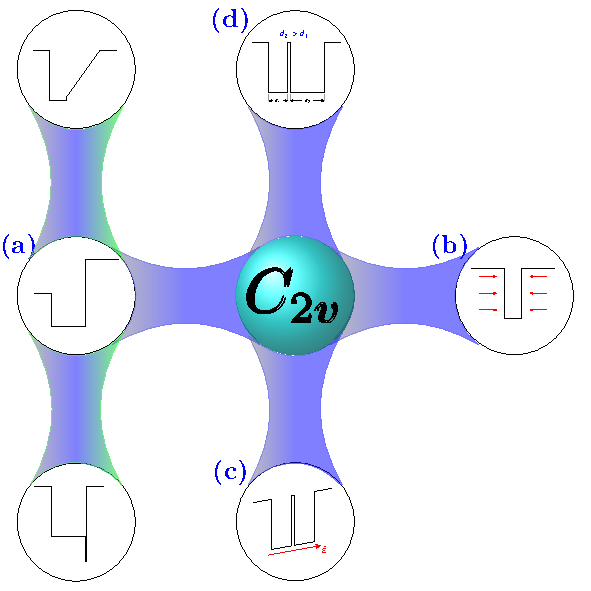
\includegraphics[width=\textwidth]{../figures/chapter-2/symmetry/out/roadmap}
		\phantomsubcaption\label{subfig:subsubsec:chapter-2-roadmap-a}
		\phantomsubcaption\label{subfig:subsubsec:chapter-2-roadmap-b}
		\phantomsubcaption\label{subfig:subsubsec:chapter-2-roadmap-c}
		\phantomsubcaption\label{subfig:subsubsec:chapter-2-roadmap-d}
		\phantomsubcaption\label{subfig:subsubsec:chapter-2-roadmap-e}
		\phantomsubcaption\label{subfig:subsubsec:chapter-2-roadmap-f}
	\end{subfigure}
	\caption
	{
		This roadmap it's developed around of QWs with remarkable potential profile, this mean posses a desire $C_{2v}$ symmetry. It starts with asymmetric QW \subref{subfig:subsubsec:chapter-2-roadmap-a}\cite{koopmans1998microscopic,andrada1997spin} specifically in potential, this is  due to the semiconductor difference in adjacent barriers to well. At center left \subref{subfig:subsubsec:chapter-2-roadmap-b} and bottom left\subref{subfig:subsubsec:chapter-2-roadmap-c} are asymmetric QWs, in the first case the asymmetry\cite{english2013effect,eldridge2011spinorbit} it's caused by gradied concentration in a barrier and bottom while the other case the asymmetry it's originated by insert an atom specie different of the barrier\cite{yu2015tuning}. At top center \subref{subfig:subsubsec:chapter-2-roadmap-d}, it's show the QW under strain\cite{english2011strain,tang2009well-width,li2019quantitative} which causes the reducing symmetry, while at bottom center\subref{subfig:subsubsec:chapter-2-roadmap-e} it shows the CQWs under applying electric field\cite{kwok1992giant}, the relation of both, it's the external perturbation which causes the breaking symmetry.  Finally, at right \subref{subfig:subsubsec:chapter-2-roadmap-f} it's presented the ACQWs which has a symmetry breaking due to the relative width of QWs\cite{ruiz2021optical}.  
	}
	\label{fig:subsubsec:chapter-2-special-symmetry--roadmap}
\end{figure}


Continued with the map, they have the perturbed structures, they are called like that due to they are under an external perturbation, at center top \Cref{subfig:subsubsec:chapter-2-roadmap-d} it's outlined a QW structure under strain applied, while at bottom center \Cref{subfig:subsubsec:chapter-2-roadmap-e} it's showing a QW structure under electric field applied. So that, in both exists, an external perturbation which causes a losses symmetry. Finally, it displays the ACQWs structure\Cref{subfig:subsubsec:chapter-2-roadmap-f}, in comparison with all above. It's notably that this structures  has two wells which are coupled by a thin barrier, by this reason as called Coupled Quantum Wells. Then, which is the reason by these structures are novels?.   

To discuss this answer, it's important to mention the relevance of CQWs being that  these structures are recurrent studied to observe quantum phenomena as exciton  (\gls{x}) condensation\cite{butov1994condensation,butov2002towards,grosso2009excitonic}. It's to be expected that in CQWs can measure indirect transitions, this means that in comparison with a single QWs whereby exists direct transitions  (band to band) hardly can measure these. But, the reality of the importance of CQWs being that excitons are very interested to apply in semiconductor devices, the properties of excitons and their interactions really exhibit quantum attractive properties. So,  unlike with single QW in CQWs the life of excitons increases\cite{hammack2009kinetics,golub1990longlived}, in fact, this is one of the principal reasons which that are attractive structures\cite{butov1994condensation,sivalertporn2012direct,winbow2011electrostatic}. Also, in terms of spin properties, the CQWs exhibit great potential\cite{bravo2022photoluminiscence}. Therefore, it being can discuss several interesting quantum properties in comparison that single structures. But, in comparison between CQWs, the symmetric structures need it perturbed to them exhibit these properties, while asymmetric structures are an excellent platform to study quantum properties such as holes mixing, spin, etc.  
It's then \emph{ACQWs an interesting structure which part from being artificial, to get natural perturbation\footnote{Thanks Dr. Raul for magnificent description.}}, even though, as can see doesn't are the unique structures with ``natural perturbation'' which generates a symmetry breaking, all above mentioned it's reduced to confinement way. This, is the reason to call special symmetry reduction in a structure hardly studied in several sub-areas of solid state. 


\section{Numerical Calculations}
\label{sec:chapter-2-numerical-calculations}
\vspace{-10mm} 
All the above cool properties mentioned, could not have been predicted or observed without their knowing their electronic properties. This is many times mentioned, is the fingerprint of semiconductors, so, also mentioned the problem to calculate it. Here was implemented a \emph{simple} model-based in \gls{efa} method to calculate the confined energies in \gls{CQWs} structures. Before explaining the numerical method to obtain these solutions, it is important to discuss the reason which can apply this method, so, it starts with the definition of band-edge from energy dispersion. In \Cref{subsec:chapter-1-valence-and-conduction-bands} are discussed in general the oncept of \gls{VB} and \gls{CB}, also is mentioned the significant methods to calculate them, in case of a heterostructure as \gls{CQWs} the complexity is greater than bulk case. In bulk, the case is well-known several methods to calculate bandstructure, where all of them are developed by the symmetry properties of the system at stake. In the case of the heterostructure, the symmetry is also important, the problem is developed a Hamiltonian capable to describe all of the system, this means, building a Hamiltonian which considers all properties as symmetry, perturbations, and in this case the potential. This work is very hard, even though exists general Hamiltonians to heterostructures, these don't warranty the correct solutions. The history and development of methods and techniques to calculate electronic properties is an area in constant evolution, from the fifties with Kane\cite{kane1957bandstructure}, Luttinger and Kohn\cite{Luttinger1955motion} in perturbed methods as \gls{kp} to Slater and Koster\cite{slater1954simplified} which proposed an atomistic method based on a linear combination of atomic orbitals called as \gls{TB}, all of this already discussed and mentioned. So, we developed a model to calculate the confined energies in coupled structures. Even though exist analytical methods to calculate confined energies, in case of CQWs is more difficult to get an exact analytical method, while also exist some analytical methods under approximation description\cite{yariv1985approximate,fromherz1997floquet,rosencher2002optoelectronics}. In the \Cref{subsection:chapter-1-preliminary-approach-of-quantum-confinment-effect-in-qws} it's developed the analytical solution of a simple quantum well taken into account the \gls{efa} method. It's possible to use this type of methods due to the symmetry reduction from bulk to QW, this due to the split in \gls{VB} which passes from being a fourfold degenerate to be a twofold degenerate. It's precisely in \gls{VB} where is it complicated to solved it. 




\subsection{Finite Difference Method}






\section{Anisotropy model in CQWs \label{sub:chap2-anisotropy-model}}

